%!TEX root = uiuc_2018_invitational.tex
\begin{problem}{Common Mistake}
{stdin}{stdout}
{1 second}{}{}

\begin{wrapfigure}{r}{0.35\textwidth}
    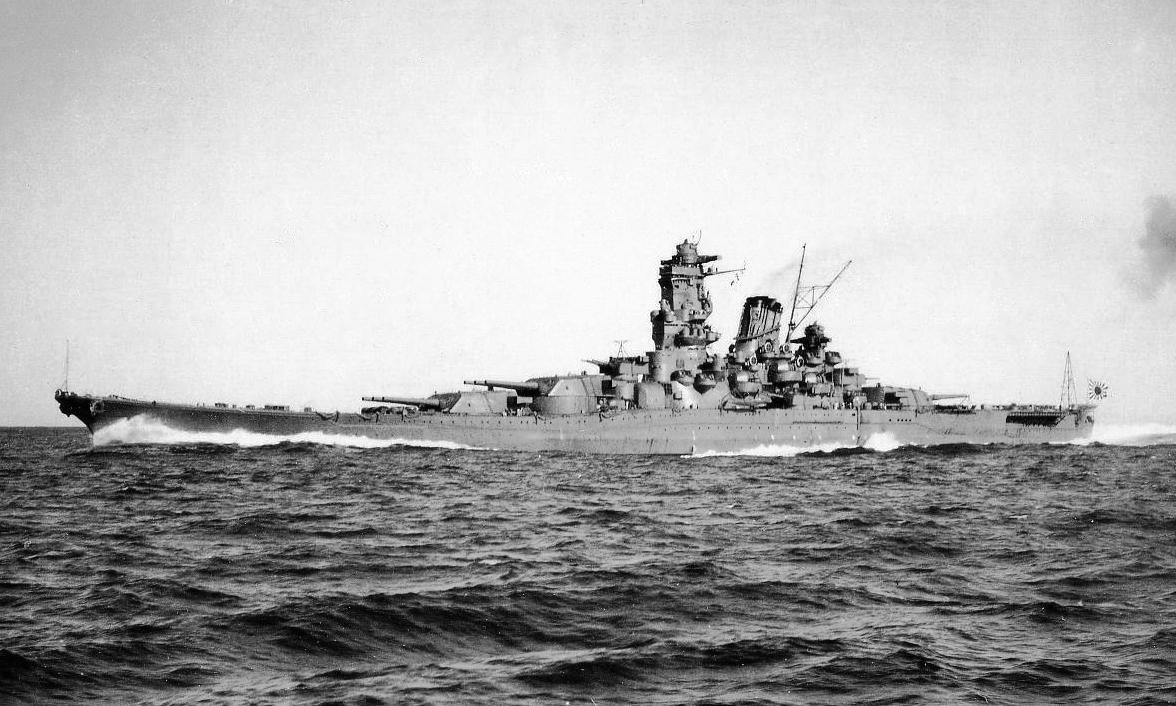
\includegraphics[scale=0.3]{yamato.jpg}
    \caption*{Yamato with her 9x46cm guns}
\end{wrapfigure}

In the era of dreadroughts and battleships, people love to stack as many guns as
possible onto warships to increase their fire power.

However, this is a common mistake. Adding too many guns will decrease
maneuverability and mobility, and ends up decreasing the overall battle
efficiency of the ships. 

Given an array of $N$ guns available, your are in charge of making the optimal
selection so the battle efficiency of a ship is maximized.

You are given the following simplified model:

Each gun will have a weight $w_i$ and power $p_i$.

The ship has $K$ load ranges. While the total weight of all guns selected is in
load range $[l_i, r_i]$, the battle efficiency of the ship is calculated as
$m_i\sum_j p_j$ where $m_i$ is the modifier associated with that load range, and
$j$ denotes the indices of all selected guns.

Note $m_i$ will not necessarily decrease as $l_i$ goes up,
because having more guns will also bring crew members pride and increase their 
morale. This in turn will bring up the battle efficiency of the whole ship.

\InputFile

The first line of input contains one integer $N (1 \le 200)$, the number 
of guns available.

In the next $N$ lines, each line will contain two nonnegative integers,
$w_i, p_i (1 \le w_i, p_i \le 100)$.

The next line contains one integer $K(2\le K \le 200)$, 
the number of load ranges.

In the next $K$ lines, each line contains two numbers $l_i, m_i$, the 
first integer is the starting weight $l_i (0 \le l_i \le 20000)$ of this load 
range.
The second number is the power modifier $m_i (0 \le m_i \le 10)$.

It is guaranteed the load ranges will be given in the increasing order 
of $l_i$, so $l_0$ will always be 0.

It is also guaranteed the last load range will always have power modifier $0$, 
which can be considered as right past the maximum load capacity of this ship.

\OutputFile

A single line with an number giving the maximum battle efficiency of the ship.
The floating number is \textbf{rounded up to 3 digits after decimal points}. 

\Examples

\begin{example}
\exmp{
3
10 30
20 40
20 40
4
0 1.0
20 2.5
50 1.8
60 0
}{%
200.000
}%
\exmp{
2
100 100
200 200
2
0 2.5
10 0
}{%
0.000
}%
\end{example}
\end{problem}
